\documentclass[crop,tikz]{standalone}
\usepackage{tikz}

\usepackage{xcolor}
\definecolor{spot}{cmyk}{1, 0.20, 0, 0}
\definecolor{comp}{cmyk}{0, 0.52, 1.0, 0}
\renewcommand{\familydefault}{\sfdefault}
\usepackage{helvet}
\usepackage{upgreek}
\usepackage[helvet]{sfmath}
\usepackage{sansmathfonts}
\usepackage{amsmath}
%\everymath={\sf}
\tikzset{
  every node/.style={
    text=black!66
  }
}
\usetikzlibrary{angles}

\usetikzlibrary{decorations.pathmorphing}

\begin{document}

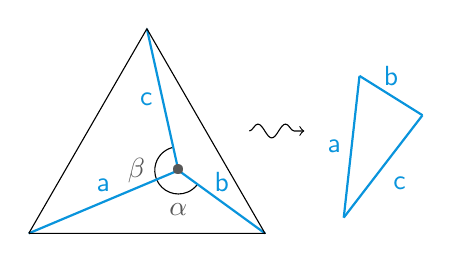
\begin{tikzpicture}
    %\draw[gray, very thin] (-3,-3) grid (3,3);

    \coordinate (P) at (1.9,.8);
    \coordinate (la) at (0,0);
    \coordinate (lb) at (0:3);
    \coordinate (lc) at (60:3);
    \pic [draw, angle radius=.3cm] {angle = la--P--lb};
    \pic [draw, angle radius=.3cm] {angle = lc--P--la};

    \draw [spot,thick] (P) -- (0,0) node [spot,midway,anchor=south] {a};
    \draw [spot,thick] (P) -- (0:3) node [spot,midway,anchor=south] {b};
    \draw [spot,thick] (P) -- (60:3) node [spot,midway,anchor=east] {c};
    \draw (0,0) -- (0:3) -- (60:3) -- (0,0);
    \node[anchor=north,yshift=-.3cm] at (P) {$\mathrm{\alpha}$};
    \node[anchor=east,xshift=-.3cm] at (P) {$\beta$};
    \draw (P) node {\textbullet};

    \draw [->, decorate, decoration=snake] (2.8,1.3) -- (3.5,1.3);

    \coordinate (A) at (4,.2);
    \coordinate (B) at (5, 1.5);
    \coordinate (C) at (4.2, 2);
    \draw [spot,thick] (A) -- (B) node [spot, anchor=north west, midway] {c};
    \draw [spot, thick] (B) -- (C) node [spot, anchor=south, midway] {b};
    \draw [spot,thick] (C) -- (A) node [spot, anchor=east, midway] {a};
\end{tikzpicture}

\end{document}